\colorlet{outlinecolor}{icyblue}

\colorlet{headercolor}{outlinecolor}
\colorlet{rowcolor1}{outlinecolor!70}
\colorlet{rowcolor2}{outlinecolor!50}


\begin{tikzpicture}
	\node [mybox, fill=boxcolor, draw=outlinecolor] (box){%
		\begin{minipage}{0.3\textwidth}
			\vspace{0.1cm}
			
			\underline{Introduction}: The \textcolor{outlinecolor}{Git stash} command allows you to temporarily save and store changes in your working directory that are not ready to be committed. It stores these changes as a \textcolor{outlinecolor}{stack data structure}. 
			\begin{itemize}
				\item \textit{When to use?} Whenever you want to save but not commit incomplete work. e.g., switching branches or addressing urgent tasks
				\item \textit{Best practices.} Save your stash with a specific stash message, especially when working with multiple stashes at once
			\end{itemize}
			
			\vspace{-3mm}
			\begin{center}
				\textcolor{background}{
					\begin{tabularx}{\textwidth}{>{\columncolor{rowcolor1}}X|>{\columncolor{rowcolor2}}p{4cm}}
						\arrayrulecolor{boxcolor} % Table line color
						\rowcolor{headercolor} % Header row color
						\multicolumn{1}{c|}{\centering \textbf{Git Command}} & \multicolumn{1}{c}{\centering \textbf{Description}} \\ % Center the header text
						\hline % Add a horizontal line below the header row
						\rowcolor{rowcolor1}
						\tablebash{git stash list} & Get the list of all stashed changes in your repo \\
						\rowcolor{rowcolor2} % New Row
						\tablebash{git stash} & Stash all tracked changes \\
						\rowcolor{rowcolor1} % New Row
						\tablebash{git stash -u} & Include untracked changes in your stash \\
						\rowcolor{rowcolor2} 
						\tablebash{git stash show stash\{\@1\}} & Shows aggregate file changes for 1st index in Git stash stack \\
						\rowcolor{rowcolor1} 
						\tablebash{git stash push -m "stash message"} & Stash your work with a clear message \\
					\end{tabularx}
				}
			\end{center}
			
			\underline{Move stashes}: Eventually, you'll either \textbf{(a)} want to delete your stashed work to declutter the stash stack or \textbf{(b)} move your stashed work back into the working directory.
			\vspace{-2mm}
			\begin{center}
				\textcolor{background}{
					\begin{tabularx}{\textwidth}{>{\columncolor{rowcolor1}}X|>{\columncolor{rowcolor2}}p{4cm}}
						\arrayrulecolor{boxcolor} % Table line color
						\rowcolor{headercolor} % Header row color
						\multicolumn{1}{c|}{\centering \textbf{Git Command}} & \multicolumn{1}{c}{\centering \textbf{Description}} \\ % Center the header text
						\hline % Add a horizontal line below the header row
						\rowcolor{rowcolor1} % New Row
						\tablebash{git stash apply} & Applies most recent stash to working directory \textbf{without deleting it} from stash stack \\
						\rowcolor{rowcolor2} 
						\tablebash{git stash drop} & Manually delete most recent stash from stack\\
						\rowcolor{rowcolor1} % New Row
						\tablebash{git stash pop} & Shorthand combination of \tablebash{git stash apply} and \tablebash{git stash drop} \\
						\rowcolor{rowcolor2}
						\tablebash{git stash apply stash\@\{1\}} & Apply a specify specific stash to working dir \\
						\rowcolor{rowcolor1}
						\tablebash{git stash drop stash\@\{1\}} & Delete a specify specific stash from stack \\
						\rowcolor{rowcolor2} 
						\tablebash{git stash clear} & Deletes all stashes \\
					\end{tabularx}
				}
			\end{center}
			\vspace{-2mm}
			
%			\underline{Stash into another branch}: You can use git stash to move changes from one branch into another one. Here are the 2 steps:
%			\begin{enumerate}
%				\item Stash the changes that you want move
%				\item Use the command \inlinebash{git stash branch new\_branch\_name} to automatically create a new branch, where your stash is applied. Your stash will also be removed from the stack.
%			\end{enumerate}
%			\vspace{-2mm}


			%			\begin{minipage}{\textwidth}
				%				\centering
				%%				\vspace{-2mm}
				%				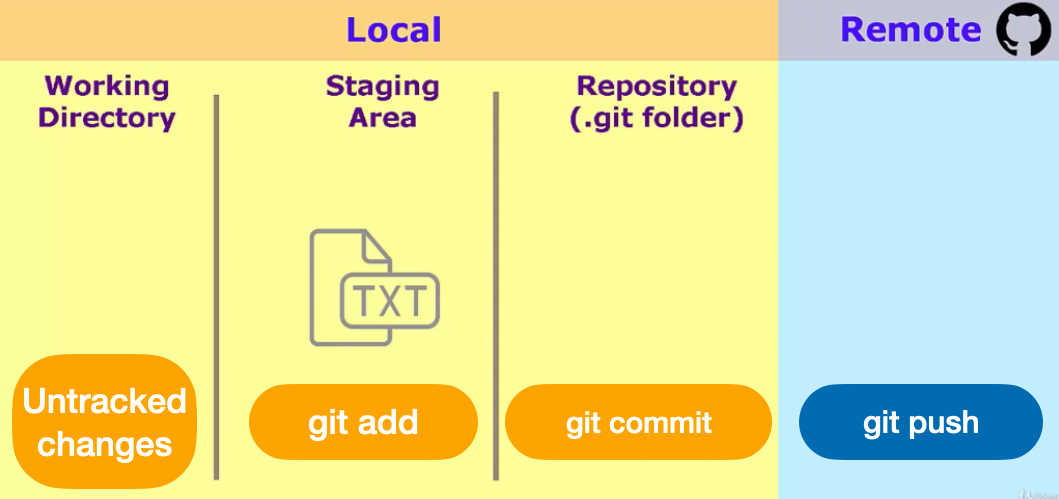
\includegraphics[width=0.5\textwidth]{images/git_stages.png}
				%				\vspace{-2mm}
				%				\captionof{figure}{Git states and associated commands. \href{https://www.udemy.com/course/git-complete/}{ \faLink{}  Source}}
				%			\end{minipage}
			
		\end{minipage}
	};
	\node[fancytitle, right=10pt, fill=outlinecolor, text=background, draw=outlinecolor, rounded corners] at (box.north west) {Stashing};
\end{tikzpicture}


\begin{tikzpicture}
	\node [mybox, fill=boxcolor, draw=outlinecolor] (box){%
		\begin{minipage}{0.3\textwidth}
			\vspace{0.1cm}
			
				\underline{Stash into another branch}: You can use git stash to move changes from one branch into another one. Here are the 2 steps:
				\begin{enumerate}
						\item Stash the changes that you want move
						\item Use the command \inlinebash{git stash branch new\_branch\_name} to automatically create a new branch, where your stash is applied. Your stash will also be removed from the stack.
				\end{enumerate}
			
			
			%			\begin{minipage}{\textwidth}
				%				\centering
				%%				\vspace{-2mm}
				%				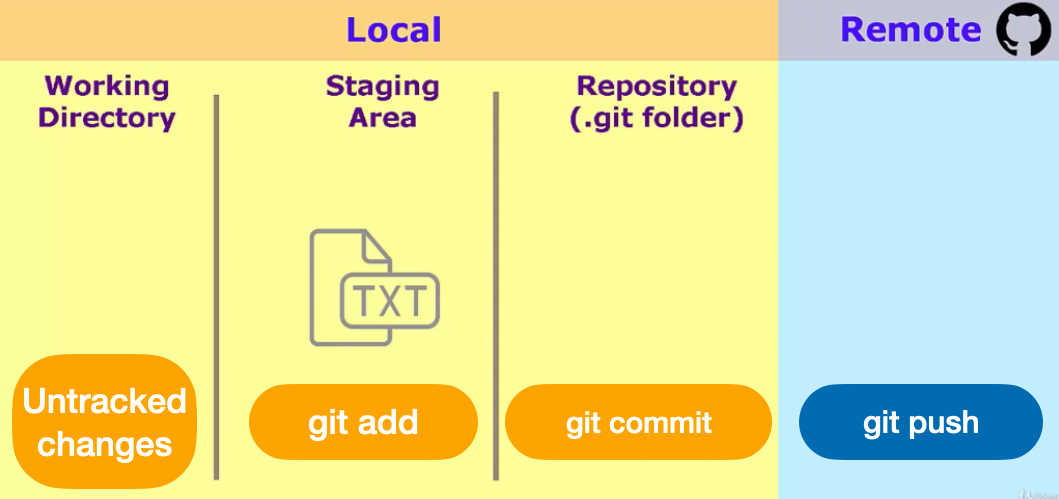
\includegraphics[width=0.5\textwidth]{images/git_stages.png}
				%				\vspace{-2mm}
				%				\captionof{figure}{Git states and associated commands. \href{https://www.udemy.com/course/git-complete/}{ \faLink{}  Source}}
				%			\end{minipage}
			
		\end{minipage}
	};
	\node[fancytitle, right=10pt, fill=outlinecolor, text=background, draw=outlinecolor, rounded corners] at (box.north west) {Stashing (2)};
\end{tikzpicture}